This chapter describes and discusses the results of the running time measurements of the cluster and baseline implementations as described in \ref{chap:implementation}. In addition, ranking accuracy results are included to validate the correctness of the Learning to Rank algorithm implementations.
\section{ListNet}
\subsection{Ranking accuracy}
\begin{table}[!h]
\centering
\begin{tabular}{p{6cm}p{1.6cm}p{1.4cm}r}\toprule
Dataset & RankLib & Cluster & Official evaluation \\
\midrule
OHSUMED (LETOR 3.0 version)     & 0.29          &   TODO & 0.3793 \\
MQ2008      					& 0.3865        &   TODO & 0.4689 \\
MQ2007      					& 0.2873        &   TODO & 0.4767 \\
MSLR-WEB10K 					& 0.1744     	&   TODO & - \\
MSLR-WEB30K 					& 0.1837     	&   TODO & - \\
\bottomrule
\end{tabular}
\caption{\acs{nDCG}@10 performance on the testing set on the first fold}
\label{tbl:accuracy_comparison}
\end{table}

\subsection{Speedup}
Figure \ref{fig:listnet_train_time} (linear data size axis) and Figure \ref{fig:listnet_train_time_log} (logarithmic data size axis) show the processing times of a single iteration of the ListNet training algorithm, using the ListNet implementation included in the RankLib library as well as the cluster implementation described in chapter \ref{chap:implementation} with different numbers of data nodes. The horizontal positions of the measurements are identical between execution method, as they are originate from the data sizes of the datasets used. Measurements were performed on a set of datasets consisting of the LETOR 3.0 OHSUMED dataset, LETOR 4.0 datasets and the MSLR-WEB10/30K datasets are used, supplemented with generated datasets that are multiplications of MSLR-WEB30K (as described in section \ref{ssec:rq2_methodology}). Table \ref{tbl:recap_datasets} describes the datasets used in the experiments and their single training fold data sizes.\\

\begin{table}[!h]
\centering
\begin{tabular}{p{3.4cm}p{3.4cm}r}\toprule
Dataset & Collection & Single fold training size \\
\midrule
MINI		& GENERATED		  & 143.38 KB\\
OHSUMED     & LETOR 3.0       &   4.55 MB\\
MQ2008      & LETOR 4.0       &   5.93 MB\\
MQ2007      & LETOR 4.0       &  25.52 MB\\
MSLR-WEB10K & MSLR-WEB10K     & 938.01 MB\\
MSLR-WEB30K & MSLR-WEB30K     &   2.62 GB\\
CUSTOM-2	& GENERATED		  &   5.25 GB\\
CUSTOM-5	& GENERATED		  &  13.12 GB\\
CUSTOM-10	& GENERATED		  &  26.24 GB\\
CUSTOM-20   & GENERATED       &  52.42 GB\\
CUSTOM-50	& GENERATED		  & 131.21 GB\\
CUSTOM-100	& GENERATED		  & 262.41 GB\\
\bottomrule
\end{tabular}
\caption{Description of datasets used for running time experiments}
\label{tbl:recap_datasets}
\end{table}

Figures \ref{fig:listnet_train_time} and \ref{fig:listnet_train_time_log} show that the single-machine RankLib implementation of ListNet is very fast compared to the Hadoop MapReduce cluster implementation of ListNet for datasets that fit in memory. As soon as the amount of data processed with RankLib ListNet approaches the physical memory limit of the machine that is used for computation (16 GB for our single-machine measurements), RankLib ListNet processing time start to increase exponentially. This increase is likely to be a result of the machine needing to use the on-disk sections of virtual memory and the swapping that takes place as a result thereof. As an exception to the datasets described in Table \ref{tbl:recap_datasets}, the largest dataset processed with RankLib ListNet is CUSTOM-8, which is 20.99 GB in size and thereby larger than the 16 GB physical memory limit. Experiments with RankLib ListNet on CUSTOM-10 were attempted, but were stopped after not completing within 12 hours. In section \ref{sec:goals} we defined speed-up as Sun and Gustafson \emph{relative speed-up} metric \cite{Sun1991} (as stated in section \ref{sec:goals}), which defines speed-up as the number of times that the execution of the fastest single machine solution is lower than the execution time with $N$ machines. Note that speed-up, following this definition, is not computable for larger datasets, as it is not computationally feasible to perform computation on datasets larger than CUSTOM-8 with a single machine. As an alternative, Figure \ref{fig:speedup_train_time} shows visualises speed-up by plotting cluster size against training time.\\


\begin{figure}[!h]
\centering
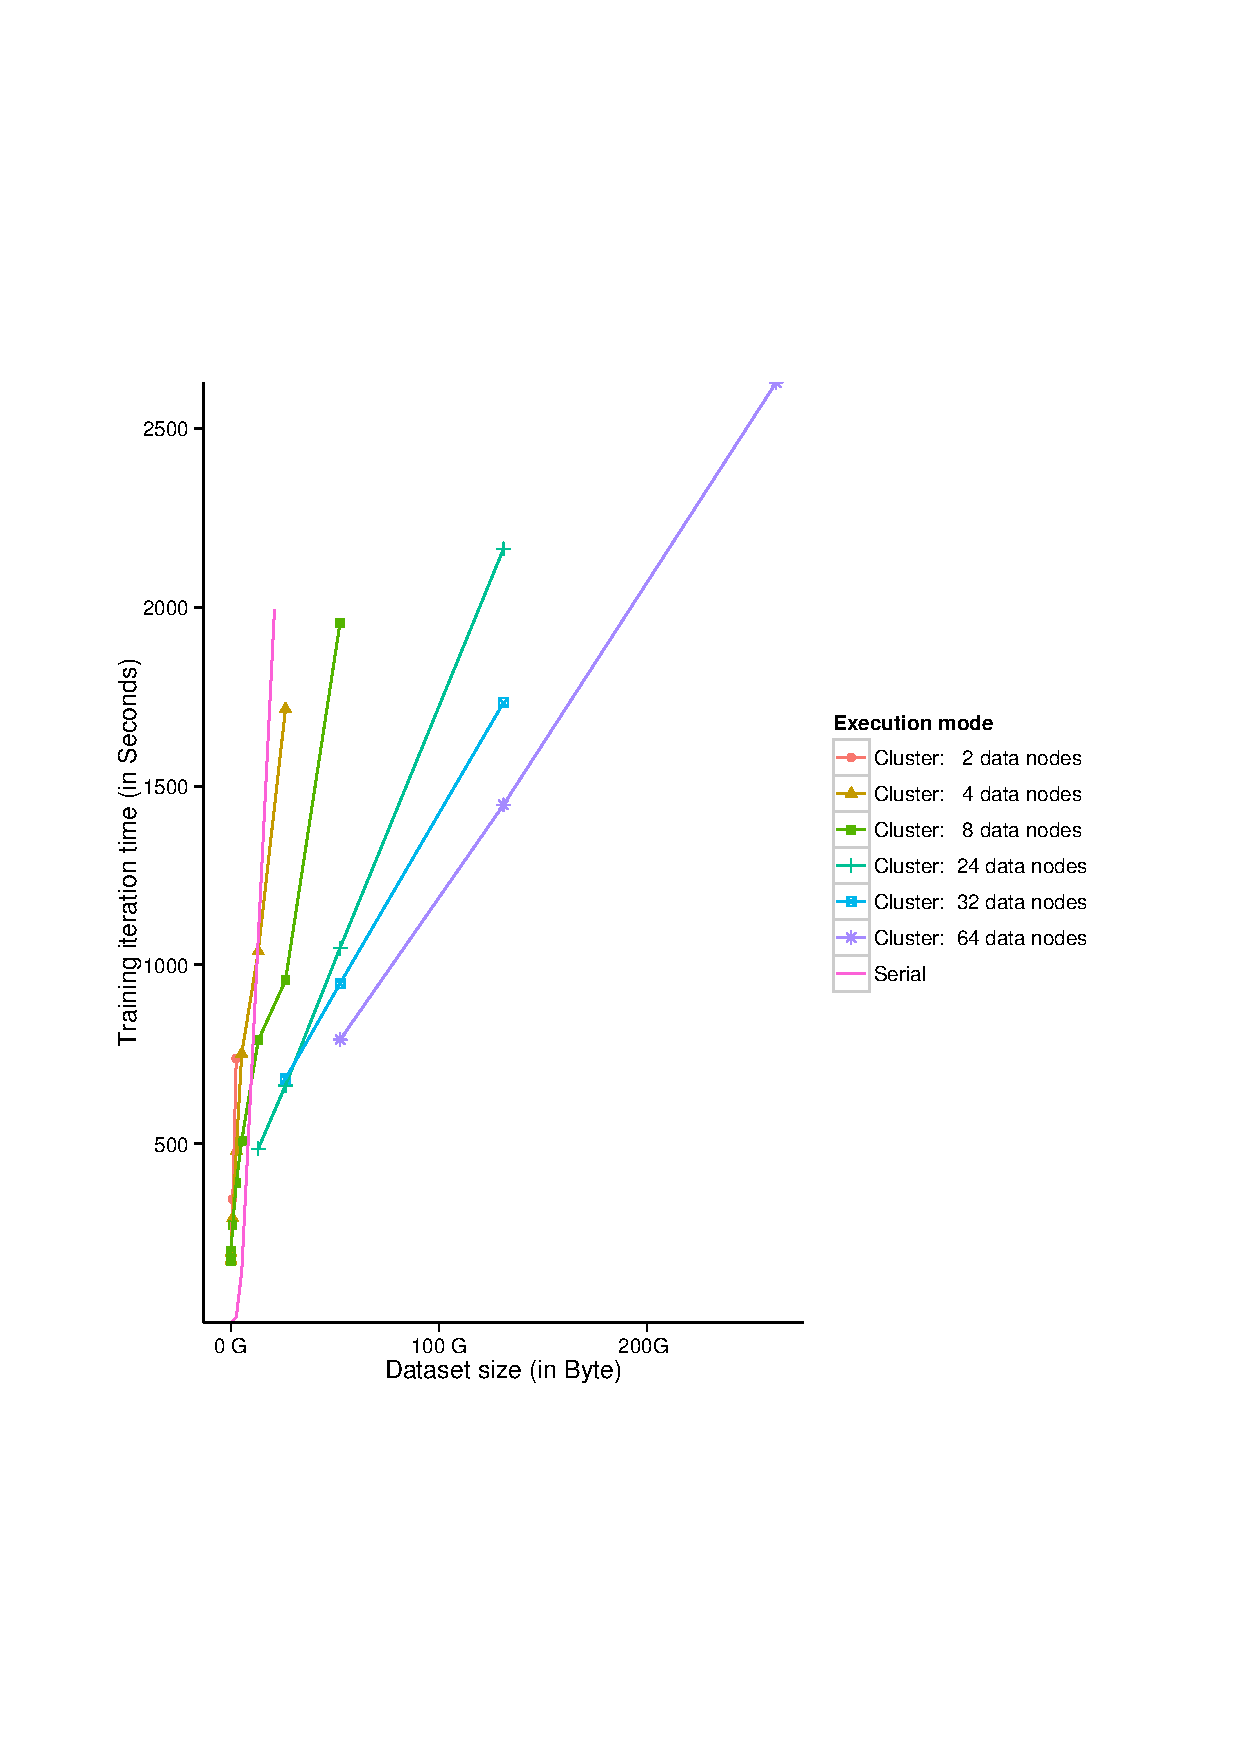
\includegraphics[trim=0cm 5cm 0cm 5cm, scale=0.8]{gfx/time_single.pdf}
\caption{Processing time of a single ListNet training iteration}
\label{fig:listnet_train_time}
\end{figure}

\begin{figure}[!h]
\centering
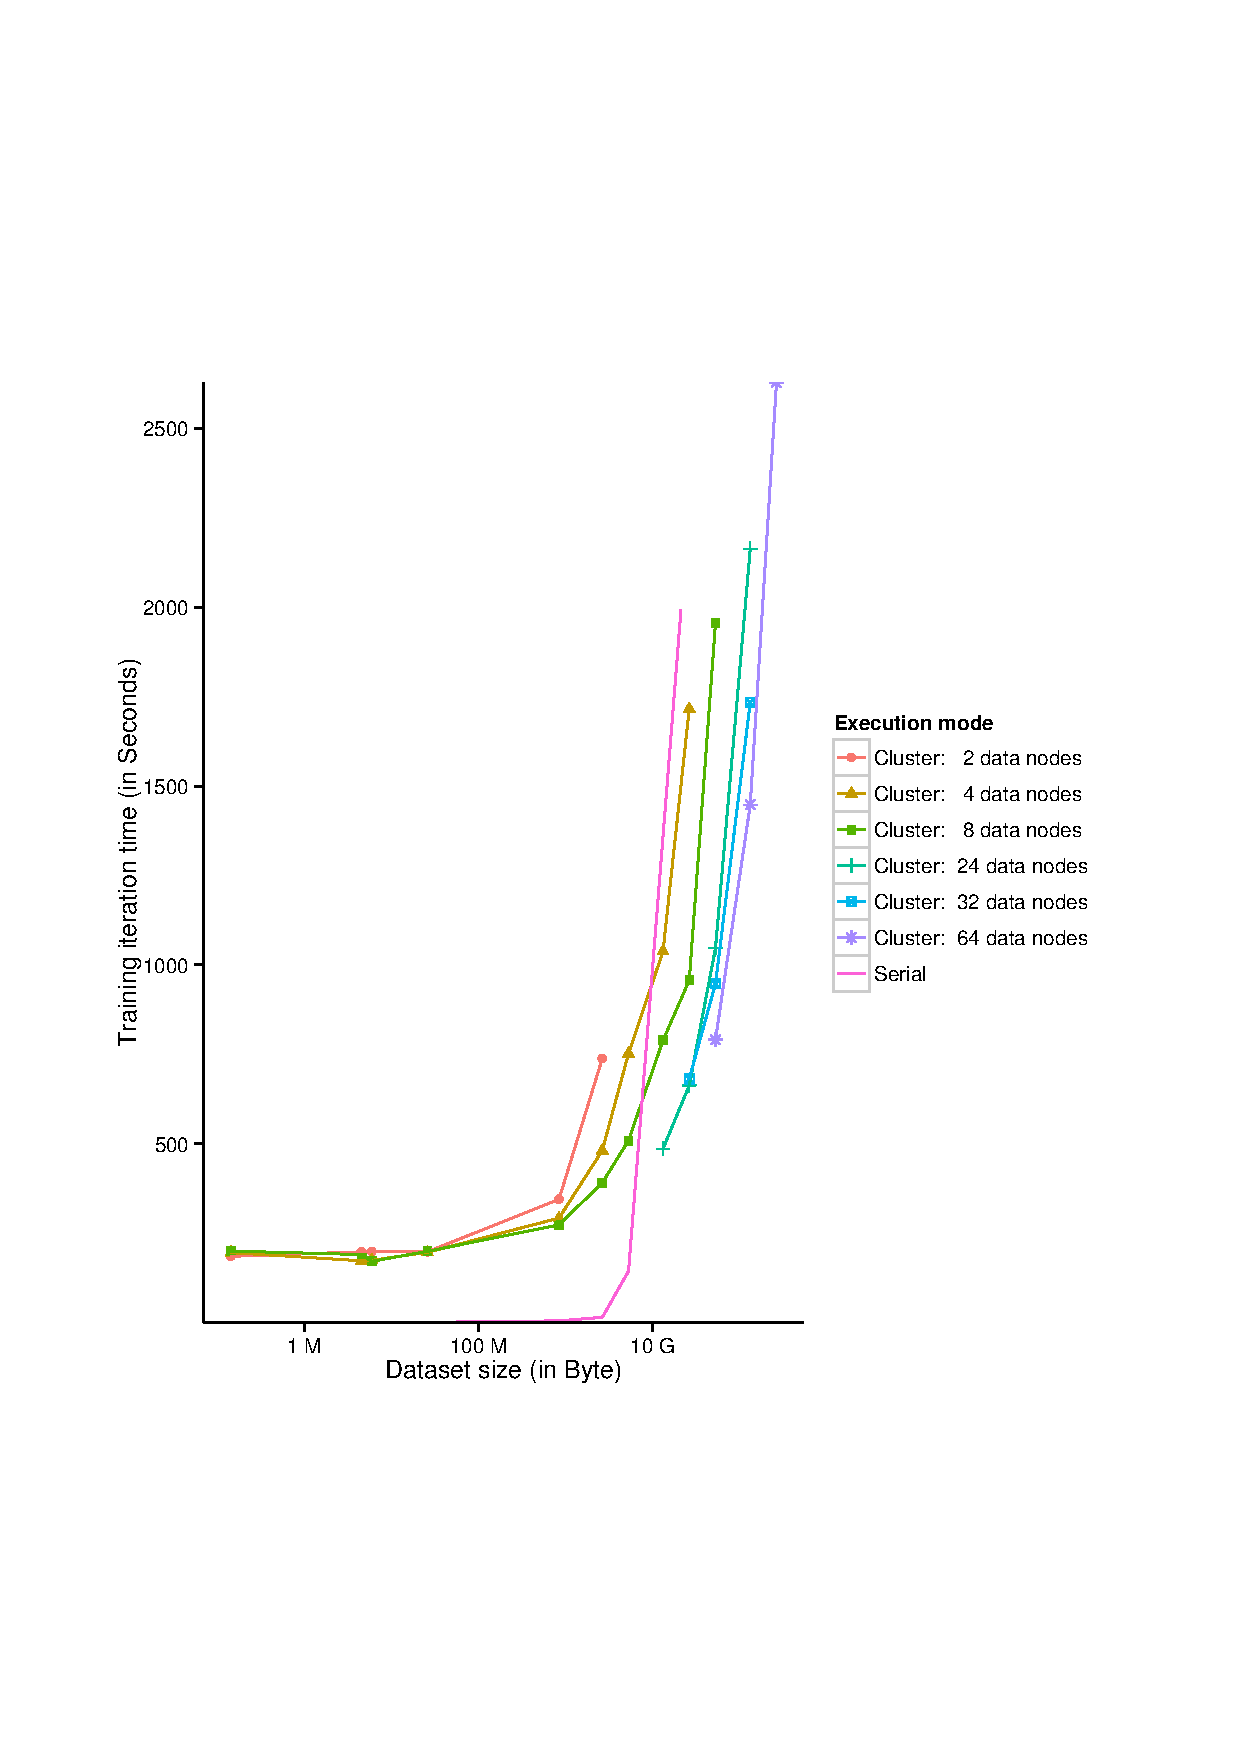
\includegraphics[trim=0cm 5cm 0cm 5cm, scale=0.8]{gfx/time_single_logx.pdf}
\caption{Processing time of a single ListNet training iteration on a logarithmic axis}
\label{fig:listnet_train_time_log}
\end{figure}

Figure \ref{fig:speedup_train_time} shows that speed-up is sub-linear, from which we can deduct that the training time converges to a constant unit of time. Based on our measurements on the small datasets MINI, OHSUMED, MQ2008 and MQ2007, this constant time seems to be within the range of 150 to 200 seconds. This time is likely to be caused by Hadoop job scheduling overhead, this presumption is strengthened by long waiting periods between the separate MapReduce jobs that form a training iteration.\\

Amdahl's law states that the speed-up of a program using parallel computing is limited by the time needed for the sequential fraction of the program. A consequence of Amdahl's Law is that all parallel programs that have a non-parallelisable part have sub-linear speed-up. Behaviour in accordance with Amdahl's law can be seen in Figure \ref{fig:speedup_train_time}, where the speed-up is sub-linear as a result of the existence a non-parallelisable fraction of the program.\\

Note however that Hadoop job scheduling overhead is independent of dataset size. Therefore, the non-parallelisable fraction of the program will be smaller when the to be processed dataset is larger, allowing larger speed-up values for larger datasets. From this observation we can derive that for \emph{"large enough"} datasets, the speed-up obtained by parallelising ListNet using Hadoop MapReduce is large enough for the parallelisation to be beneficial in terms of processing time compared to the RankLib single-machine version of ListNet, even when the size of the to be processed dataset would not have been memory-bounded in RankLib ListNet.\\

Figure \ref{fig:listnet_throughput} shows the throughput in bytes per second. Our observation that RankLib ListNet performs very slow for data sets that do not fit in physical memory and virtual memory is needed is very notable in this graph. Furthermore, this graph shows how both increase in number in data nodes in a cluster and increase in input data size result in an increase in throughput. The sub-linear growth of throughput as a factor of input data size can again be explained as a result of the non-parallelisable Hadoop job scheduling part of the operation.\\

\begin{figure}[!h]
\centering
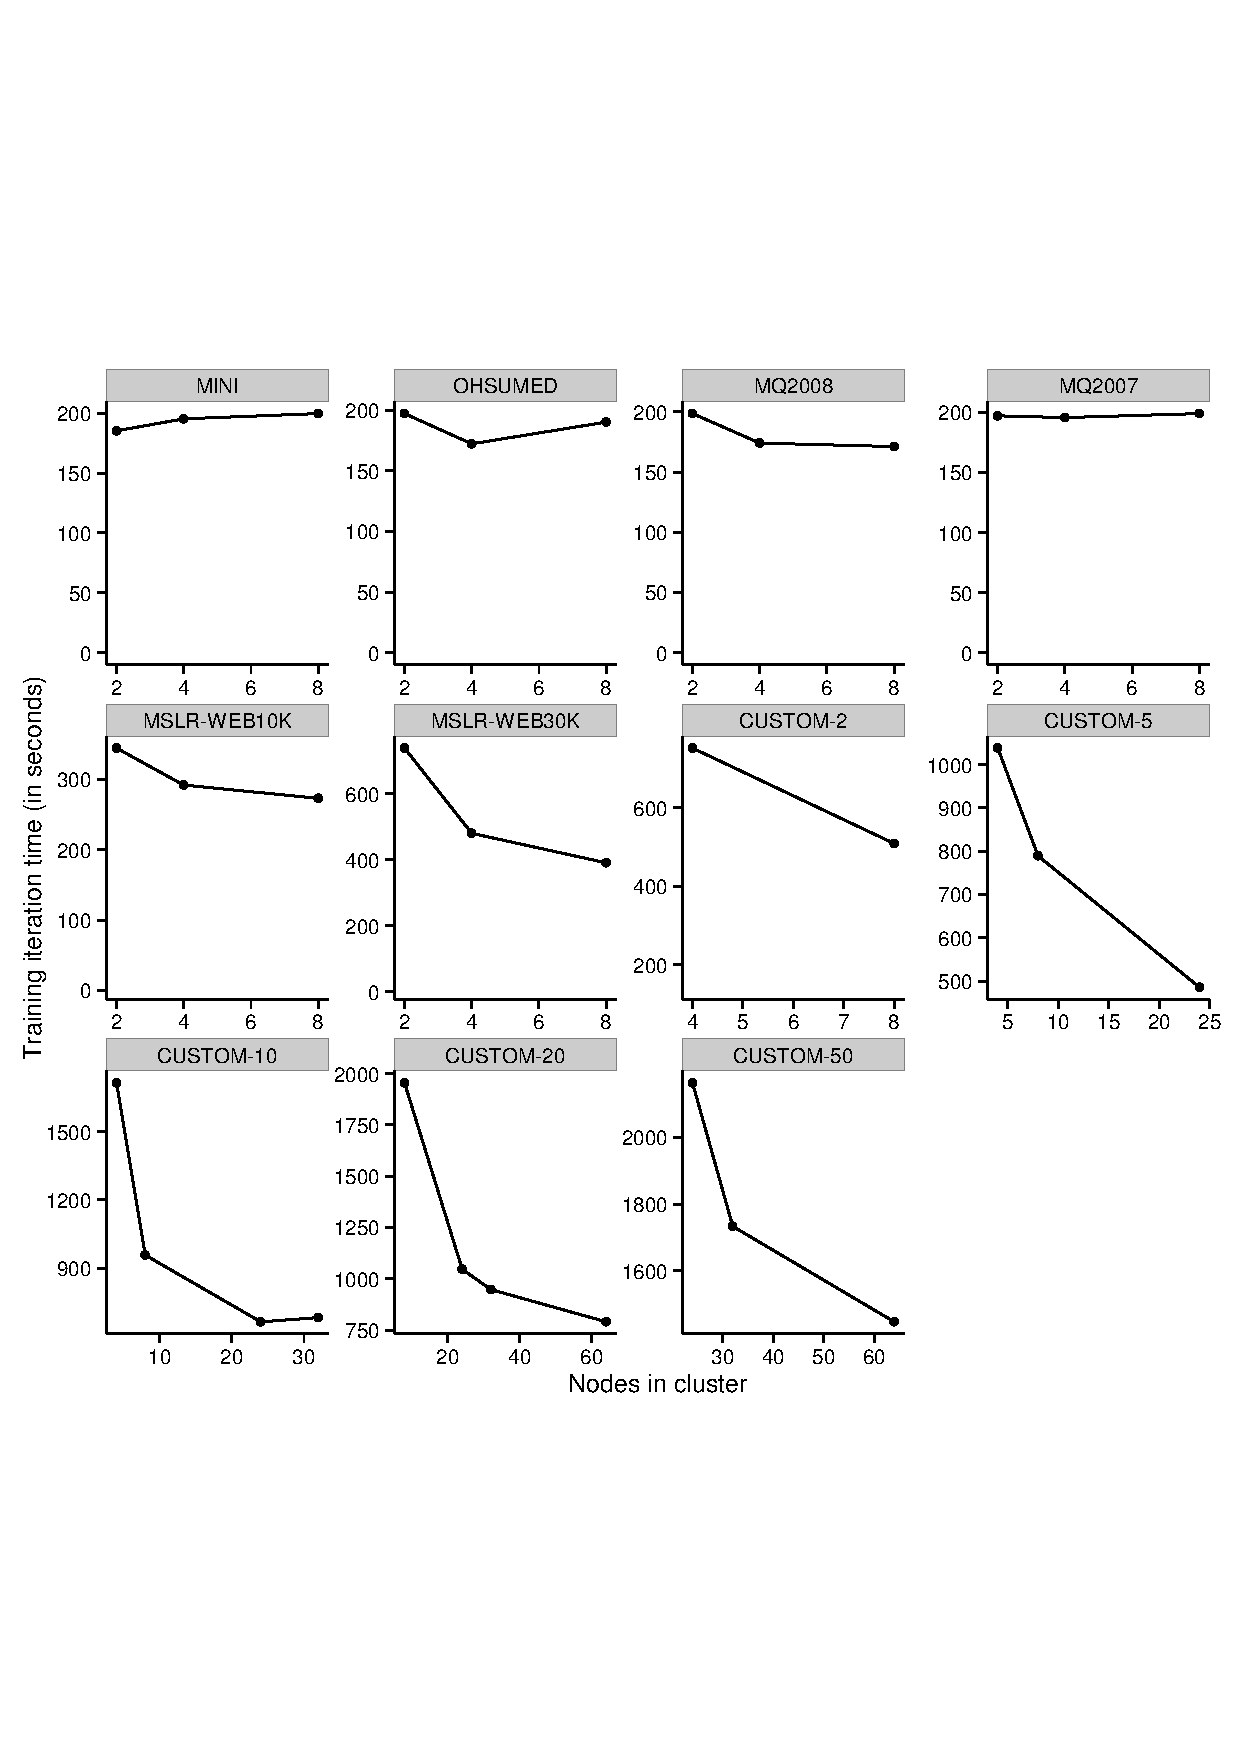
\includegraphics[trim=0cm 5cm 0cm 5cm, scale=0.7]{gfx/speedup_faceted.pdf}
\caption{Processing time as a function of data nodes in a cluster}
\label{fig:speedup_train_time}
\end{figure}

\begin{figure}[!h]
\centering
\includegraphics[trim=0cm 5cm 0cm 5cm, scale=0.8]{gfx/throughput_single_logx.pdf}
\caption{Throughput of a ListNet training iteration}
\label{fig:listnet_throughput}
\end{figure}